\newpage
\section{Model-to-tree transformation with TGGs}
\genHeader

{\huge REMOVE}

One powerful benefit of working with TGG transformations is that by specifiying one transformation (i.e., a forward transformation), we're able to get the
opposite direction for free! Our example used a \texttt{tree.xmi} (\texttt{MocaTree}
instance) input, transformed it forward into \texttt{tree.xmi\_fwd.xmi} (\texttt{Dictionary} instance), and used that result file in a backwards
transformation to create the final tree output, \texttt{tree.xmi\_FWD.xmi\_BWD.xmi}, all without error! If our TGG was truly successful however,
the starting and final files should be identical. Let's compare the two (Fig.~\ref{eclipse:comparingTreeModels}).

It's close, but not perfect. You can see that some things need to be refined. The ``DICTIONARY'' and ``ENTRY'' labels, for example, are missing from the
major nodes. We need to include an attribute constraint to bind these specific EString values. You'll also notice that, as you scroll through each
\texttt{Node}, the \texttt{title} and \texttt{author} nodes have the correct \texttt{index} values of 0 and 1, but the remaining \texttt{entry} indices are also
set to 0. We were only concerned with binding the title and author nodes in the forward direction, as we could assume that any other node with any other index
value (2 and greater) was an \texttt{entryNode}. In the backwards direction however, this distinction is lost, which means we must introduce a custom attribute constraint.

\jumpDual{m2tvis}{m2ttex}

\newpage
\hypertarget{m2ttex}{}
\subsection{Refining the TGG Transformation}
\texHeader

\begin{itemize}

\item[$\blacktriangleright$] Find the relevant files and add the following attribute constraints. Note : the MOSL parser requires that all attribute constraints
are declared before link variables.

\begin{figure}[htp]
\begin{center}
  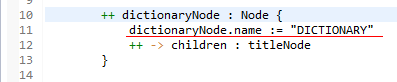
\includegraphics[width=0.8\textwidth]{eclipse_NodeToDictionaryRule_updated}
  \caption[labelInTOC]{needs refinement\ldots}
  \label{eclipse:generatedBkwrdMdl}
\end{center}
\end{figure}

\begin{figure}[htp]
\begin{center}
  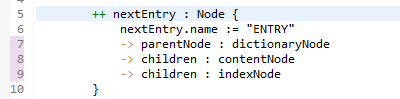
\includegraphics[width=0.8\textwidth]{eclipse_ForAllEntryRule_updated}
  \caption[labelInTOC]{needs refinement\ldots}
  \label{eclipse:generatedBkwrdMdl}
\end{center}
\end{figure} 

\item[$\blacktriangleright$] Add new SetDefaultNumber CSP here.

\begin{figure}[htbp]
\begin{center}
  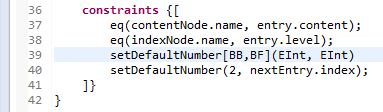
\includegraphics[width=0.6\textwidth]{eclipse_setDefaultNumberConstraint}
  \caption{extra constraint}
  \label{eclipse:newEntryConstraint}
\end{center}
\end{figure}

\end{itemize}

